\documentclass[english,usenames,dvipsnames]{beamer}
\usetheme{default}
\beamertemplatenavigationsymbolsempty
\setbeamertemplate{footline}[frame number]
\setbeamercolor{alerted text}{fg=blue1}
%\setbeamercolor{frametitle}{fg=blue2}
\usepackage[utf8]{inputenc}
\usepackage{caption}
\usepackage{booktabs}
\usepackage{appendixnumberbeamer}
\usepackage{babel}
\usepackage{amsmath}
\usepackage{hyperref}
\usepackage{geometry}
\usepackage{bbm}
\usepackage{tikz}
\usepackage{amsthm}
\usepackage{verbatim}
%\usepackage{palatino}
\definecolor{red1}{RGB}{155,50,0}
\definecolor{blue1}{RGB}{0,0,155}
\definecolor{blue2}{rgb}{0.22,0.37,1}
\definecolor{green1}{RGB}{34,139,35}

\setbeamertemplate{itemize items}[default]


\title{Noncompete Agreements and Endogenous Growth with Creative Destruction}
\author{Nicolas Fernandez-Arias}
\date{\today }

\begin{document}

\maketitle

\section{Introduction}

\begin{frame}{Notes from talk}
\begin{itemize}
	\item Richard: not clear what my main narrative is
	\item Richard: calibrating without NCAs, so be clear about what model I'm solving etc. and what data I'm using 
	\item Richard: who founds spinouts? What are their positions? how am I interpreting that it's related to R\&D?
	\item Continue to tighten up model presentation...kind of confusing. just do the presentation over and over again to more people.
	\item Variation in mechanism by NCA enforceability? 
	\item Selection: Venture Source vs. firms not in Venture Source
	\item Highlight what the main takeaways of firm type comparison
	\item Patents held by entrepreneurs -- who founds firms, even if not R\&D? so try to match
	\item What difference when trying match incumbent relative R\&D spending instead of patents
	\item Be explicit about what you're showing in calibation: i.e., need to be more explicit about how things only depend on $m$ etc
	\item Stats about non-competes at the beginning to motivate the non-competes
	\item no caveats before results
	\item Motivation (channel) and then model, then empirics
	\item Don't put $\kappa$ discussion in presentation
	\item Efficiency of R\&D very different between incumbents and entrants -- does literature agree? Compare to literature
	\item Put motivation figure first, then model, then dive into empirics more carefully to discpline model, then calibration
	\item Do exercise of just selling paper with no caveats
	\item Add little picture explaining where entry comes from, add narrative, etc. Be a bit more defensive of paper (to practice job talk)
	\item Have answer for "what happens if startup is in different state from previous employer?"
\end{itemize}
\end{frame}

\begin{frame}{Motivation 1}
\begin{itemize}
	\item Firm entry contributes substantially to productivity growth
	\item Growth due to firm entry largely due to creative destruction, rather than new product varieties
	\item Important source of successful new firms is \alert{\textbf{within-industry spinouts (WSOs)}}
	\begin{itemize}
		\item Entering firm whose founders previously worked in same industry 
		\hyperlink{spinouts_facts_from_literature}{\beamergotobutton{stylized facts}}
		\item Fairchild semiconductor descendents \hyperlink{fairchildren_early}{\beamergotobutton{graphic}}
	\end{itemize}
\end{itemize}
\end{frame}

\begin{frame}{Motivation 2}
\begin{itemize}
	\item Productivity is developed through \alert{\textbf{R\&D investment}}
	\item Hypothesis: entrepreneurs bring \alert{\textbf{\textbf{knowledge acquired at previous employers}}} to their new firms
	\item Entry by WSOs \alert{\textbf{increases competition}}
	\item Implication: entry by WSOs can \alert{\textbf{reduce expected payoff}} of incumbent R\&D investments $\Rightarrow$ GE effect \alert{\textbf{reduces incumbent innovation}}
\end{itemize}
\end{frame}

\begin{frame}{Motivation 3}
\begin{itemize}
	\item \alert{\textbf{Non-compete agreements (NCAs)}} allow employees of incumbent firms to commit not to form WSOs
	\item GE effects of creative destruction by WSOs $\Rightarrow$ NCAs may increase incumbent innovation, aggregate productivity growth and welfare
	\item Ongoing \alert{\textbf{policy debate}}
	\begin{itemize}
		\item Silicon Valley success (in particular, relative to Massachusetts Route 128) often attributed to California's \alert{\textbf{non-enforcement of NCAs}}
		\item States passing laws restricting enforcement of noncompetes (Hawaii in 2015, Massachussetts and Maryland in 2019, several others)
	\end{itemize}
\end{itemize}
\end{frame}

\begin{frame}{This project}
\begin{itemize}
	\item Question: what is the effect of non-compete agreements on aggregate productivity growth and welfare?
	\item Empirics of spinouts
	\begin{itemize}
		\item R\&D leads to formation of more WSOs
		\item WSOs have more revenue, are larger, more valuable, more likely to be acquired / IPO, less likely to fail than ordinary firms
		\item Qualitatively same holds for \alert{\textbf{other-industry spinouts (OSOs)}}
	\end{itemize}
	\item GE model of endogenous growth where incumbent firm \alert{\textbf{R\&D generates ideas for employee spinouts}}
	\item Calibration to match micro empirics and aggregate data
	\item Policy exercise: allowing noncompetes \alert{\textbf{increases welfare}} by 1.25\% 
\end{itemize}
\end{frame}

\begin{frame}{Related literature}
\begin{itemize}
\item Firm dynamics and endogenous growth
\begin{itemize}
\item Romer 1986, Grossman \& Helpman 1991, Aghion \& Howitt 1992, Klette \& Kortum 2004, Acmemoglu \& Akcigit 2012, Akcigit \& Kerr 2017
\end{itemize}
\item Models of employee spinouts
\begin{itemize}
\item Klepper 2002, Klepper \& Sleeper 2005, Anton \& Yao 1994/1995, Franco \& Filson 2006, Franco \& Mitchell 2008, Rauch 2015, Rossi-Hansberg \& Chatterjee 2012
\item Baslandze 2019
\end{itemize}
\item Empirics on employee mobility, spinouts
\begin{itemize}
\item Spawning of spinouts: Gompers et al. 2005, Garmaise 2011, Baslandze 2019, Babina \& Howell 2019
\item Characteristics of spinouts: Muendler 2012
\item Effect on parent firms: Campbell et. al 2012, Wezel et al. 2006
\item Effect of non-compete enforcement: Garmaise 2009, Marx et al 2009, Samila-Sorenson 2011, Jeffers 2018, Shi 2018
\end{itemize}
\end{itemize}
\end{frame}



\section{Empirics}

\begin{frame}
\tableofcontents[currentsection]
\end{frame}

\begin{frame}{Venture Source}
\begin{itemize}
	\item Deal and company data for US-based startups funded by VCs from 1986-2008
	\item 23,008 startups, 147,516 individuals, 89,382 financing rounds
	\item Valuation, IPO / M\&A, employment, revenue, business failure
	\item \textbf{\alert{Key feature: }} employment biographies for founders / C-level / board members
\end{itemize}
\end{frame}

\begin{frame}{Merging with Compustat and patent data}
\begin{itemize}
\item Match individuals Venture Source to previous employers in Compustat using employment biographies
\item NBER-USPTO patent data
\begin{itemize}
	\item Data on all USPTO-registered patents and their citations (also data on inventors, associated firms)
\end{itemize}
\end{itemize}
\end{frame}

\begin{frame}{Results of match to Compustat}
\begin{figure}
	\includegraphics[scale=0.23]{figures/presentation/table1_founder2.png}
\end{figure}
\end{frame}

\begin{frame}{Corporate R\&D and spinout formation}
\begin{figure}[!htb]
	\centering
	\includegraphics[scale= 0.4]{../empirics/figures/scatterPlot_RD-Founders_dIntersection.png}
	\caption{Scatterplot of average yearly founder counts in $t+1,t+2,t+3$ versus average yearly R\&D spending in $t,t-1,t-2$.}
\end{figure}
\end{frame}

\begin{frame}{Corporate R\&D and WSO formation}

\begin{figure}[!htb]
\centering
\includegraphics[scale= 0.4]{../empirics/figures/scatterPlot_RD-FoundersWSO4_dIntersection.png}
\caption{Scatterplot of average yearly WSO4 founder counts in $t+1,t+2,t+3$ versus average yearly R\&D spending in $t,t-1,t-2$.}
\end{figure}
\end{frame}

\begin{frame}{Corporate R\&D and spinout formation regression: OLS specification 1}
\begin{table}
\Tiny
\centering
{
\def\sym#1{\ifmmode^{#1}\else\(^{#1}\)\fi}
\begin{tabular}{l*{8}{c}}
\toprule
                    &\multicolumn{1}{c}{(1)}&\multicolumn{1}{c}{(2)}&\multicolumn{1}{c}{(3)}&\multicolumn{1}{c}{(4)}&\multicolumn{1}{c}{(5)}&\multicolumn{1}{c}{(6)}&\multicolumn{1}{c}{(7)}&\multicolumn{1}{c}{(8)}\\
                    &\multicolumn{1}{c}{Founders}&\multicolumn{1}{c}{Founders}&\multicolumn{1}{c}{Founders}&\multicolumn{1}{c}{Founders}&\multicolumn{1}{c}{WSO4}&\multicolumn{1}{c}{WSO4}&\multicolumn{1}{c}{WSO4}&\multicolumn{1}{c}{WSO4}\\
\midrule
R\&D                &        0.34\sym{**} &        0.73\sym{***}&        0.73\sym{***}&        0.63\sym{***}&        0.19\sym{***}&        0.32\sym{***}&        0.31\sym{***}&        0.28\sym{***}\\
                    &      (0.13)         &      (0.24)         &      (0.23)         &      (0.14)         &     (0.045)         &     (0.067)         &     (0.065)         &     (0.050)         \\
\addlinespace
No FE               &         Yes         &          No         &          No         &          No         &         Yes         &          No         &          No         &          No         \\
\addlinespace
Firm FE             &          No         &         Yes         &         Yes         &         Yes         &          No         &         Yes         &         Yes         &         Yes         \\
\addlinespace
Year FE             &          No         &         Yes         &          No         &          No         &          No         &         Yes         &          No         &          No         \\
\addlinespace
Age FE              &          No         &          No         &         Yes         &          No         &          No         &          No         &         Yes         &          No         \\
\addlinespace
Industry-Age FE     &          No         &          No         &          No         &         Yes         &          No         &          No         &          No         &         Yes         \\
\addlinespace
Industry-Year FE    &          No         &          No         &         Yes         &          No         &          No         &          No         &         Yes         &          No         \\
\addlinespace
State-Year FE       &          No         &          No         &         Yes         &          No         &          No         &          No         &         Yes         &          No         \\
\addlinespace
Industry-State-Year FE&          No         &          No         &          No         &         Yes         &          No         &          No         &          No         &         Yes         \\
\midrule
r2\_a                &        0.24         &        0.69         &        0.69         &        0.75         &        0.21         &        0.65         &        0.64         &        0.61         \\
r2\_a\_within         &        0.24         &        0.26         &        0.26         &        0.24         &        0.21         &        0.25         &        0.23         &        0.15         \\
N                   &       65009         &       63732         &       62211         &       37810         &       65009         &       63732         &       62211         &       37810         \\
\bottomrule
\multicolumn{9}{l}{\footnotesize Standard errors in parentheses}\\
\multicolumn{9}{l}{\footnotesize \sym{*} \(p<0.1\), \sym{**} \(p<0.05\), \sym{***} \(p<0.01\)}\\
\end{tabular}
}

\caption{\tiny The dependent variable is average yearly number of founders joining startups in years $t+1,t+2,t+3$. The independent variables are averages over $t,t-1,t-2$. Firm controls are employment, assets, intangible assets, investment, net income, cumulative citation-weighted patents, and the product of Tobin's Q and Assets. Standard errors are clustered by firm.}
\end{table}
\end{frame}

\begin{frame}{Corporate R\&D and spinout formation regression: OLS specification 2}
\begin{table}
\Tiny
\centering
{
\def\sym#1{\ifmmode^{#1}\else\(^{#1}\)\fi}
\begin{tabular}{l*{8}{c}}
\toprule
                    &\multicolumn{1}{c}{(1)}&\multicolumn{1}{c}{(2)}&\multicolumn{1}{c}{(3)}&\multicolumn{1}{c}{(4)}&\multicolumn{1}{c}{(5)}&\multicolumn{1}{c}{(6)}&\multicolumn{1}{c}{(7)}&\multicolumn{1}{c}{(8)}\\
                    &\multicolumn{1}{c}{$\frac{\textrm{Founders}}{\textrm{Assets}}$}&\multicolumn{1}{c}{$\frac{\textrm{Founders}}{\textrm{Assets}}$}&\multicolumn{1}{c}{$\frac{\textrm{Founders}}{\textrm{Assets}}$}&\multicolumn{1}{c}{$\frac{\textrm{Founders}}{\textrm{Assets}}$}&\multicolumn{1}{c}{$\frac{\textrm{WSO4}}{\textrm{Assets}}$}&\multicolumn{1}{c}{$\frac{\textrm{WSO4}}{\textrm{Assets}}$}&\multicolumn{1}{c}{$\frac{\textrm{WSO4}}{\textrm{Assets}}$}&\multicolumn{1}{c}{$\frac{\textrm{WSO4}}{\textrm{Assets}}$}\\
\midrule
$\frac{\textrm{R\&D}}{\textrm{Assets}}$&        1.71\sym{***}&        1.12         &        1.15         &        0.28         &        0.82\sym{***}&        0.62\sym{**} &        0.57         &        0.77         \\
                    &      (0.34)         &      (0.68)         &      (0.71)         &      (1.05)         &      (0.17)         &      (0.32)         &      (0.36)         &      (0.88)         \\
\addlinespace
NAICS4-State-Age-Year FE&          No         &          No         &          No         &         Yes         &          No         &          No         &          No         &         Yes         \\
\addlinespace
NAICS4-Year FE      &          No         &          No         &         Yes         &          No         &          No         &          No         &         Yes         &          No         \\
\addlinespace
State-Year FE       &          No         &          No         &         Yes         &          No         &          No         &          No         &         Yes         &          No         \\
\addlinespace
Firm FE             &          No         &         Yes         &         Yes         &         Yes         &          No         &         Yes         &         Yes         &         Yes         \\
\addlinespace
Age FE              &          No         &          No         &         Yes         &          No         &          No         &          No         &         Yes         &          No         \\
\addlinespace
Year FE             &          No         &         Yes         &          No         &          No         &          No         &         Yes         &          No         &          No         \\
\addlinespace
No FE               &         Yes         &          No         &          No         &          No         &         Yes         &          No         &          No         &          No         \\
\midrule
r2\_a                &       0.014         &        0.26         &        0.22         &        0.25         &      0.0088         &        0.27         &        0.21         &        0.40         \\
r2\_a\_within         &       0.014         &      0.0028         &      0.0025         &      0.0014         &      0.0088         &      0.0014         &      0.0012         &      0.0046         \\
N                   &       60687         &       59477         &       58201         &       23665         &       60687         &       59477         &       58201         &       23665         \\
\bottomrule
\multicolumn{9}{l}{\footnotesize Standard errors in parentheses}\\
\multicolumn{9}{l}{\footnotesize \sym{*} \(p<0.1\), \sym{**} \(p<0.05\), \sym{***} \(p<0.01\)}\\
\end{tabular}
}

\caption{\tiny The dependent variable is the average yearly number of founders from the parent firm joining startups in years $t+1,t+2,t+3$, normalized by a trailing five-year moving average of assets. Independent variables are also normalized by assets. Standard errors are clustered at the firm level.}
\label{table:RDandSpinoutFormation_at_founder2_l3f3}
\end{table}
\end{frame}

\begin{frame}{Instrumenting R\&D}
\begin{itemize}
	\item Bloom, 2013: exogenous firm-specific variation in state and federal tax incentives for R\&D
	\item State-level
	\begin{itemize}
		\item Weighted average of state-level after-tax cost of R\&D based on location of last 10 years of firm's inventors
		\item Problem with exclusion restriction
	\end{itemize}
	\item Firm-level
	\begin{itemize}
		\item Firm-specific R\&D subsidy a function of firm-specific base of past R\&D spending
		\item Problem with exogeneity
	\end{itemize}
	\item LATE vs average effect
\end{itemize}
\end{frame}

\begin{frame}{Corporate R\&D and spinout formation regression: IV specification}
\begin{table}
\Tiny
\centering
{
\def\sym#1{\ifmmode^{#1}\else\(^{#1}\)\fi}
\begin{tabular}{l*{8}{c}}
\toprule
                    &\multicolumn{1}{c}{(1)}&\multicolumn{1}{c}{(2)}&\multicolumn{1}{c}{(3)}&\multicolumn{1}{c}{(4)}&\multicolumn{1}{c}{(5)}&\multicolumn{1}{c}{(6)}&\multicolumn{1}{c}{(7)}&\multicolumn{1}{c}{(8)}\\
                    &\multicolumn{1}{c}{Founders}&\multicolumn{1}{c}{Founders}&\multicolumn{1}{c}{Founders}&\multicolumn{1}{c}{Founders}&\multicolumn{1}{c}{WSO4}&\multicolumn{1}{c}{WSO4}&\multicolumn{1}{c}{WSO4}&\multicolumn{1}{c}{WSO4}\\
\midrule
log(R\&D)           &        0.19\sym{***}&        0.84\sym{+}  &       -0.94         &        0.38         &        0.18\sym{***}&       -0.92         &        1.08\sym{*}  &        0.14         \\
                    &     (0.022)         &      (0.53)         &      (8.21)         &      (0.58)         &     (0.026)         &      (4.68)         &      (0.61)         &      (0.76)         \\
\addlinespace
highNCC=0 $\times$ log(R\&D)&           0         &           0         &           0         &           0         &           0         &           0         &           0         &           0         \\
                    &         (.)         &         (.)         &         (.)         &         (.)         &         (.)         &         (.)         &         (.)         &         (.)         \\
\addlinespace
highNCC=1 $\times$ log(R\&D)&       0.033         &       -1.32         &        3.85         &       -0.21         &       0.018         &        3.16         &        0.20         &     -0.0060         \\
                    &     (0.053)         &      (1.45)         &      (18.3)         &      (0.67)         &     (0.069)         &      (12.3)         &      (0.73)         &      (0.53)         \\
\addlinespace
NAICS4-Year FE      &          No         &          No         &          No         &         Yes         &          No         &          No         &          No         &         Yes         \\
\addlinespace
Firm FE             &         Yes         &         Yes         &         Yes         &         Yes         &         Yes         &         Yes         &         Yes         &         Yes         \\
\addlinespace
Firm Age FE         &          No         &          No         &         Yes         &         Yes         &          No         &          No         &         Yes         &         Yes         \\
\addlinespace
Year FE             &          No         &          No         &         Yes         &          No         &          No         &          No         &         Yes         &          No         \\
\midrule
r2\_a                &        0.68         &       -0.58         &       -1.96         &       -0.30         &        0.60         &       -3.98         &       -0.12         &       -0.27         \\
r2\_a\_within         &       0.099         &                     &                     &                     &        0.12         &                     &                     &                     \\
N                   &        7111         &        4007         &        1206         &         909         &        2950         &        1675         &         467         &         389         \\
\bottomrule
\multicolumn{9}{l}{\footnotesize Standard errors in parentheses}\\
\multicolumn{9}{l}{\footnotesize \sym{++} \(p<0.3\), \sym{+} \(p<0.2\), \sym{*} \(p<0.1\), \sym{**} \(p<0.05\), \sym{***} \(p<0.01\)}\\
\end{tabular}
}

\caption{\tiny The dependent variable is the log of the average yearly number of founders from the parent firm joining startups, over the years $t+1,t+2,t+3$. Independent variables are similarly averaged over $t,t-1,t-2$. Columns (1) and (5) are estimated by OLS. The remaining columns columns are estimated by instrumenting R\&D spending using firm-specific tax incentives for R\&D, from Bloom 2013. Standard errors are clustered at the firm level.}
\label{table:RDandSpinoutFormation_iv_founder2_l3f3}
\end{table}
\end{frame}

\begin{frame}{Defining spinout firms in the data}
\begin{itemize}	
	\item WSO has at least one founder in same 4-digit NAICS industry as previous employer
	\item OSO has at least one founder matched to Compustat, but none in the same 4-digit NAICS industry
\end{itemize}
\end{frame}

\begin{frame}{Spinouts have higher employment}
	\begin{table}
		\tiny
		\centering
		{
\def\sym#1{\ifmmode^{#1}\else\(^{#1}\)\fi}
\begin{tabular}{l*{4}{c}}
\hline\hline
                    &\multicolumn{1}{c}{(1)}         &\multicolumn{1}{c}{(2)}         &\multicolumn{1}{c}{(3)}         &\multicolumn{1}{c}{(4)}         \\
\hline
Spinout=1           &        0.31\sym{***}&        0.21\sym{***}&        0.22\sym{***}&        0.20\sym{***}\\
                    &     (0.038)         &     (0.011)         &     (0.017)         &     (0.013)         \\
[1em]
WSO4=1              &       0.067         &        0.13\sym{***}&        0.13\sym{***}&        0.13\sym{***}\\
                    &      (0.15)         &    (0.0056)         &   (0.00040)         &    (0.0072)         \\
[1em]
Constant            &        3.14\sym{***}&        3.09\sym{***}&        3.12\sym{***}&        3.10\sym{***}\\
                    &     (0.075)         &    (0.0039)         &    (0.0052)         &     (0.012)         \\
[1em]
State-NAICS4-Year FE&          No         &         Yes         &         Yes         &          No         \\
[1em]
State-NAICS4-Age FE &          No         &         Yes         &          No         &         Yes         \\
[1em]
State-NAICS4-Cohort FE&          No         &          No         &         Yes         &         Yes         \\
[1em]
No FE               &         Yes         &          No         &          No         &          No         \\
\hline
r2\_a                &       0.012         &        0.39         &        0.46         &        0.44         \\
r2\_a\_within         &       0.012         &       0.015         &       0.014         &       0.013         \\
N                   &       54424         &       43323         &       44124         &       43802         \\
\hline\hline
\multicolumn{5}{l}{\footnotesize Standard errors in parentheses}\\
\multicolumn{5}{l}{\footnotesize \sym{*} \(p<0.1\), \sym{**} \(p<0.05\), \sym{***} \(p<0.01\)}\\
\end{tabular}
}

		\caption{\footnotesize The regresssions above compare \textbf{\alert{employment}} in WSO4 spinouts, non-WSO4 spinouts and non-spinouts. The first regression uses no controls. The following three regressions in addition control for year effects, age effects, and / or cohort effects, in each case allowing the relevant effect to differ by State-NAICS4 combination. Standard errors are multi-way clustered at the state, NAICS4 and year levels.}
	\end{table}
\end{frame}

\begin{frame}{Spinouts have higher valuations}
	\begin{table}
		\tiny
		\centering
		{
\def\sym#1{\ifmmode^{#1}\else\(^{#1}\)\fi}
\begin{tabular}{l*{4}{c}}
\hline\hline
                    &\multicolumn{1}{c}{(1)}         &\multicolumn{1}{c}{(2)}         &\multicolumn{1}{c}{(3)}         &\multicolumn{1}{c}{(4)}         \\
\hline
Spinout=1           &        0.28\sym{***}&        0.20\sym{***}&        0.18\sym{***}&        0.18\sym{***}\\
                    &     (0.066)         &     (0.043)         &     (0.037)         &     (0.046)         \\
[1em]
WSO4=1              &        0.15\sym{***}&        0.15\sym{***}&        0.13\sym{***}&        0.10\sym{***}\\
                    &     (0.047)         &     (0.017)         &   (0.00065)         &     (0.012)         \\
[1em]
Constant            &        3.51\sym{***}&        3.55\sym{***}&        3.59\sym{***}&        3.56\sym{***}\\
                    &      (0.10)         &     (0.014)         &     (0.014)         &     (0.055)         \\
[1em]
State-NAICS4-Year FE&          No         &         Yes         &         Yes         &          No         \\
[1em]
State-NAICS4-Age FE &          No         &         Yes         &          No         &         Yes         \\
[1em]
State-NAICS4-Cohort FE&          No         &          No         &         Yes         &         Yes         \\
[1em]
No FE               &         Yes         &          No         &          No         &          No         \\
\hline
r2\_a                &       0.011         &        0.31         &        0.31         &        0.29         \\
r2\_a\_within         &       0.011         &       0.012         &      0.0085         &      0.0069         \\
N                   &       26504         &       19566         &       19845         &       20823         \\
\hline\hline
\multicolumn{5}{l}{\footnotesize Standard errors in parentheses}\\
\multicolumn{5}{l}{\footnotesize \sym{*} \(p<0.1\), \sym{**} \(p<0.05\), \sym{***} \(p<0.01\)}\\
\end{tabular}
}

		\caption{\footnotesize The regresssions above compare \textbf{\alert{valuation}} in WSO4 spinouts, non-WSO4 spinouts and non-spinouts. The first regression uses no controls. The following three regressions in addition control for year effects, age effects, and / or cohort effects, in each case allowing the relevant effect to differ by State-NAICS4 combination. Standard errors are multi-way clustered at the state, NAICS4 and year levels.}
	\end{table}
\end{frame}

\begin{frame}{Spinouts have higher revenue}
\begin{table}
\tiny
\centering
{
\def\sym#1{\ifmmode^{#1}\else\(^{#1}\)\fi}
\begin{tabular}{l*{4}{c}}
\hline\hline
                    &\multicolumn{1}{c}{(1)}         &\multicolumn{1}{c}{(2)}         &\multicolumn{1}{c}{(3)}         &\multicolumn{1}{c}{(4)}         \\
\hline
WSO4                &       -0.12         &        0.43\sym{***}&        0.42\sym{***}&        0.39\sym{***}\\
                    &      (0.16)         &      (0.14)         &      (0.13)         &      (0.14)         \\
[1em]
Constant            &        1.90\sym{***}&        1.80\sym{***}&        1.84\sym{***}&        1.83\sym{***}\\
                    &      (0.14)         &     (0.010)         &    (0.0096)         &     (0.010)         \\
[1em]
State FE            &          No         &         Yes         &         Yes         &         Yes         \\
[1em]
NAICS4-Year FE      &          No         &         Yes         &         Yes         &          No         \\
[1em]
NAICS4-Age FE       &          No         &         Yes         &          No         &         Yes         \\
[1em]
NAICS4-Cohort FE    &          No         &          No         &         Yes         &         Yes         \\
[1em]
No FE               &         Yes         &          No         &          No         &          No         \\
\hline
clustvar            &statecode naics1\_4 year         &statecode naics1\_4         &statecode naics1\_4         &statecode naics1\_4         \\
r2\_a                &     0.00011         &        0.31         &        0.36         &        0.36         \\
r2\_a\_within         &     0.00011         &      0.0028         &      0.0027         &      0.0022         \\
N                   &       17838         &       16891         &       16875         &       17134         \\
\hline\hline
\multicolumn{5}{l}{\footnotesize Standard errors in parentheses}\\
\multicolumn{5}{l}{\footnotesize \sym{*} \(p<0.1\), \sym{**} \(p<0.05\), \sym{***} \(p<0.01\)}\\
\end{tabular}
}

\caption{\footnotesize The regresssions above compare \textbf{\alert{revenue}} in WSO4 spinouts, non-WSO4 spinouts and non-spinouts. The first regression uses no controls. The following three regressions in addition control for year effects, age effects, and / or cohort effects, in each case allowing the relevant effect to differ by State-NAICS4 combination. Standard errors are multi-way clustered at the state, NAICS4 and year levels.}
\end{table}
\end{frame}

\begin{frame}{Spinouts more likely to IPO / M\&A}
\begin{table}
\tiny
\centering
{
\def\sym#1{\ifmmode^{#1}\else\(^{#1}\)\fi}
\begin{tabular}{l*{4}{c}}
\toprule
                    &\multicolumn{1}{c}{(1)}         &\multicolumn{1}{c}{(2)}         &\multicolumn{1}{c}{(3)}         &\multicolumn{1}{c}{(4)}         \\
\midrule
$\frac{\text{WSO4 founders}}{\text{Total founders}}$&        2.52\sym{***}&        2.19\sym{***}&        2.03\sym{***}&        2.01\sym{***}\\
                    &     (0.056)         &      (0.14)         &      (0.18)         &      (0.18)         \\
\addlinespace
State-Year FE       &          No         &         Yes         &         Yes         &          No         \\
\addlinespace
State-Age FE        &          No         &         Yes         &          No         &         Yes         \\
\addlinespace
State-Cohort FE     &          No         &          No         &         Yes         &         Yes         \\
\addlinespace
NAICS4-Year FE      &          No         &         Yes         &         Yes         &          No         \\
\addlinespace
NAICS4-Age FE       &          No         &         Yes         &          No         &         Yes         \\
\addlinespace
NAICS4-Cohort FE    &          No         &          No         &         Yes         &         Yes         \\
\midrule
Clustering          &State, Industry         &State, Industry         &State, Industry         &State, Industry         \\
R-squared (adj.)    &     0.00046         &       0.035         &       0.033         &       0.035         \\
R-squared (within, adj)&     0.00046         &     0.00034         &     0.00027         &     0.00027         \\
Observations        &      240155         &      239696         &      239788         &      239959         \\
\bottomrule
\multicolumn{5}{l}{\footnotesize Standard errors in parentheses}\\
\multicolumn{5}{l}{\footnotesize \sym{*} \(p<0.1\), \sym{**} \(p<0.05\), \sym{***} \(p<0.01\)}\\
\end{tabular}
}

\caption{\footnotesize The regresssions above compare the \textbf{\alert{M\&A and IPO hazard rate}} in WSO4 spinouts, non-WSO4 spinouts and non-spinouts. The first regression uses no controls. The following three regressions in addition control for year effects, age effects, and / or cohort effects, in each case allowing the relevant effect to differ by State-NAICS4 combination. Standard errors are multi-way clustered at the state, NAICS4 and year levels.}
\end{table}
\end{frame}

\begin{frame}{Spinouts less likely to fail}
\begin{table}
\tiny
\centering
{
\def\sym#1{\ifmmode^{#1}\else\(^{#1}\)\fi}
\begin{tabular}{l*{4}{c}}
\toprule
                    &\multicolumn{1}{c}{(1)}         &\multicolumn{1}{c}{(2)}         &\multicolumn{1}{c}{(3)}         &\multicolumn{1}{c}{(4)}         \\
\midrule
$\frac{\text{WSO4 founders}}{\text{Total founders}}$&       -0.16         &       -0.57\sym{***}&       -0.54\sym{***}&       -0.56\sym{***}\\
                    &      (0.23)         &      (0.12)         &      (0.11)         &     (0.099)         \\
\addlinespace
Constant            &        1.59\sym{***}&        1.61\sym{***}&        1.61\sym{***}&        1.61\sym{***}\\
                    &      (0.35)         &    (0.0013)         &    (0.0023)         &    (0.0016)         \\
\addlinespace
State-Year FE       &          No         &         Yes         &         Yes         &          No         \\
\addlinespace
State-Age FE        &          No         &         Yes         &          No         &         Yes         \\
\addlinespace
State-Cohort FE     &          No         &          No         &         Yes         &         Yes         \\
\addlinespace
NAICS4-Year FE      &          No         &         Yes         &         Yes         &          No         \\
\addlinespace
NAICS4-Age FE       &          No         &         Yes         &          No         &         Yes         \\
\addlinespace
NAICS4-Cohort FE    &          No         &          No         &         Yes         &         Yes         \\
\addlinespace
No FE               &         Yes         &          No         &          No         &          No         \\
\midrule
Clustering          &statecode naics1\_4 year         &statecode naics1\_4         &statecode naics1\_4         &statecode naics1\_4         \\
R-squared (adj.)    &   0.0000015         &       0.030         &       0.032         &       0.017         \\
R-squared (within, adj)&   0.0000015         &    0.000065         &    0.000054         &    0.000057         \\
Observations        &      251910         &      251460         &      251552         &      251710         \\
\bottomrule
\multicolumn{5}{l}{\footnotesize Standard errors in parentheses}\\
\multicolumn{5}{l}{\footnotesize \sym{*} \(p<0.1\), \sym{**} \(p<0.05\), \sym{***} \(p<0.01\)}\\
\end{tabular}
}

\caption{\footnotesize The regresssions above compare the \textbf{\alert{failure rate}} in WSO4 spinouts, non-WSO4 spinouts and non-spinouts. The first regression uses no controls. The following three regressions in addition control for year effects, age effects, and / or cohort effects, in each case allowing the relevant effect to differ by State-NAICS4 combination. Standard errors are multi-way clustered at the state, NAICS4 and year levels.}
\end{table}
\end{frame}

\begin{frame}{Knowledge spillover vs selection}
\begin{itemize}
	\item No exogenous variation in assignment of employees to previous employers 
	\item Correlation with exogenous shocks to R\&D helps but not quite sufficient to establish knowledge spillovers
	\begin{itemize}
		\item Could be that future entrepreneurs move to high-R\&D firms
	\end{itemize}
	\item Babina \& Howell, 2019: employees with above-median tenure equally likely to start firms in response to R\&D spending
\end{itemize}
\end{frame}


\section{Model}

\begin{frame}
\tableofcontents[currentsection]
\end{frame}

\begin{frame}{Model}
\begin{itemize}	
\item Quality ladder model of endogenous growth through creative destruction 
\begin{itemize}
	\item Builds on Grossman-Helpman 1991, Akcigit-Kerr 2017 
\end{itemize}
\item \alert{\textbf{New:}} R\&D workers \textbf{\alert{acquire ability to form spinouts}} on the job
\begin{itemize}
	\item Flow of knowledge is \textbf{\alert{disincentive}} to incumbent R\&D
	\item Stock of disseminated knowledge is incentive to incumbent R\&D: \textbf{\alert{escape competition}} effect
\end{itemize} 
\item \alert{\textbf{New:}} Non-compete agreements
\begin{itemize}
	\item Reduce flow of knowledge, \textbf{\alert{shrinking production possibilities frontier}}
	\item \textbf{\alert{May increase welfare}} due to effect on incumbent R\&D incentives
\end{itemize}
\end{itemize}
\end{frame}


\begin{frame}{Households}
\begin{itemize}
\item Unit continuum of individuals are risk-neutral, discount rate $\rho > 0$, objective
\begin{align*}
\mathbb{E}_t \int_0^{\infty} e^{-\rho s} c_i(t+s) ds
\end{align*}
where $c_i(t)$ is household $i$ consumption of final good at time $t$
\item One unit of labor, inelastic, used in final good or intermediate good production, or R\&D
\end{itemize}
\end{frame}

\begin{frame}{Production}
\begin{itemize}
	\item \textbf{\alert{Final goods}}:
	\begin{align*}
	Y = F(L,\{q_j\},\{k_j\}) &= \frac{L_F^{\beta}}{1-\beta} \int_0^1 q_j^{\beta} k_j^{1-\beta}  dj 
	\end{align*}
	\begin{itemize}
		\item Labor $L_F$, intermediate goods $\{k_j\}$, qualities $\{q_j\}$, $j \in [0,1]$
		\item No storage
	\end{itemize}
	\item \alert{\textbf{Intermediate goods}}:
	\begin{align*}
	k_j = Q l_j
	\end{align*}
	\begin{itemize}
		\item Average quality $Q = \int_0^1 q_j dj$
	\end{itemize}
\end{itemize}
\end{frame}

\begin{frame}{Incumbent innovation}
\begin{itemize}
\item Incumbent ($I$) discovers next innovation with Poisson intensity
\begin{align*}
\tau^I(z) &= \chi_I z^{1-\psi}
\end{align*}
where $z$ is units of R\&D, $\chi_I$ is R\&D productivity, and $\psi \in (0,1)$ measures decreasing returns to R\&D 
\item Innovation increases quality by exogenous factor $\lambda > 1$
\item Scaling assumption: one unit of R\&D on quality $q$ requires $(q/Q)$ units of labor in R\&D
\end{itemize}
\end{frame}

\begin{frame}{Creative destruction}
\begin{itemize}
	\item Good $j$: mass 1 entrants (E), mass $m_j$ spinouts (S)
	\item Aggregates $z_E(j) = \int_0^1 z_E^e(j) de$, $z_S(j) = \int_0^{m} z_S^s(j) ds$
	\item Innovation technology
	\begin{align*}
	\textrm{Spinouts: }\tau^S(z,z_E+z_S) &= \chi_{S} z (z_E + z_S)^{-\hat{\psi}} \\
	\textrm{Entrants: }\tau^E(z,z_E+z_S) &= \chi_{E} z (z_E + z_S)^{-\hat{\psi}}
	\end{align*}
	\item Aggregate DRS $\hat{\psi} > \psi$ due to lack of coordination: \alert{\textbf{fishing out}} and \textbf{\alert{duplication of research}} 
	\item Spinouts have \textbf{\alert{capacity constraint}} $z_S^s \le 1$
\end{itemize}
\end{frame}

\begin{frame}{Generation of spinouts}
\begin{itemize}
\item Rate $\theta \frac{Q}{q_j} \nu$ per flow unit of labor, R\&D generates spinouts in line $j$
\item Rate $(1-\theta) \nu$, idea generated in random line $j'$
\item Conditional on no innovations, law of motion for mass of potential spinouts: $\dot{m}_j = \dot{m}_j^{\textrm{WSO}} + \dot{m}_j^{\textrm{OSO}}$ where
	\begin{align*}
	\dot{m}_j^{\textrm{WSO}}&= \theta \nu z_{I,j} (1-x_j)\\
	\dot{m}_j^{\textrm{OSO}} &= (1-\theta)\nu \int_0^1 \frac{q_j}{Q} z_{I,j'} dj'
	\end{align*}
where $x_j = 1$ if the incumbent imposes a non-compete
\item Incumbent or entrant innovates on $j$ $\Rightarrow$ $m_j$ jumps to 0
\end{itemize}
\end{frame}


\begin{frame}{Dynamics of an individual good $j$}
\begin{figure}
	\centering
	%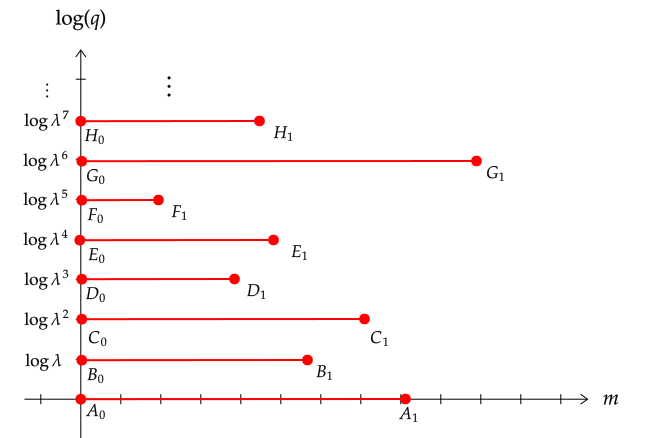
\includegraphics[scale=0.5]{figures/tikz/individual_product_line_dynamics.png}
	\resizebox{!}{.6\textheight}{

\tikzset{every picture/.style={line width=0.75pt}} %set default line width to 0.75pt        

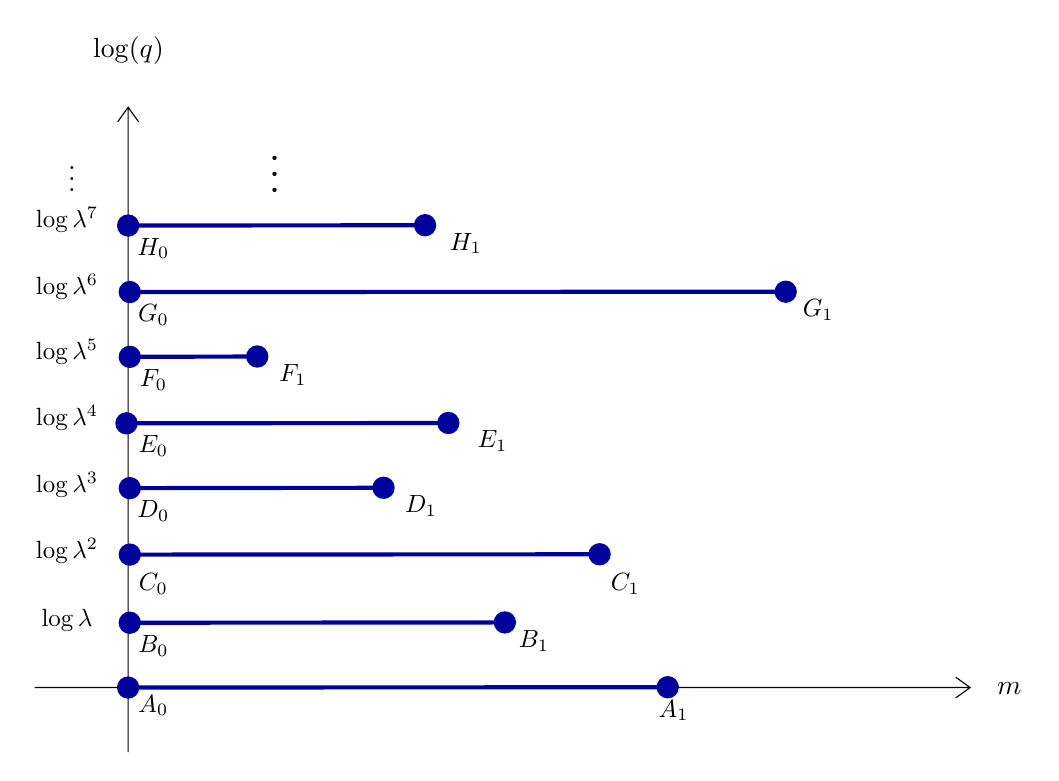
\begin{tikzpicture}[x=0.75pt,y=0.75pt,yscale=-1,xscale=1]
%uncomment if require: \path (0,436); %set diagram left start at 0, and has height of 436

%Shape: Axis 2D [id:dp5962309555056176] 
\draw  (23.9,406.93) -- (474.68,406.93)(68.98,127.34) -- (68.98,438) (467.68,401.93) -- (474.68,406.93) -- (467.68,411.93) (63.98,134.34) -- (68.98,127.34) -- (73.98,134.34)  ;
%Straight Lines [id:da5785444046568369] 
\draw [color={rgb, 255:red, 0; green, 0; blue, 155 }  ,draw opacity=1 ][line width=1.5]    (68.98,406.93) -- (328.96,406.77) ;
\draw [shift={(328.96,406.77)}, rotate = 359.96] [color={rgb, 255:red, 0; green, 0; blue, 155 }  ,draw opacity=1 ][fill={rgb, 255:red, 0; green, 0; blue, 155 }  ,fill opacity=1 ][line width=1.5]      (0, 0) circle [x radius= 4.36, y radius= 4.36]   ;
\draw [shift={(68.98,406.93)}, rotate = 359.96] [color={rgb, 255:red, 0; green, 0; blue, 155 }  ,draw opacity=1 ][fill={rgb, 255:red, 0; green, 0; blue, 155 }  ,fill opacity=1 ][line width=1.5]      (0, 0) circle [x radius= 4.36, y radius= 4.36]   ;
%Straight Lines [id:da8891623197358631] 
\draw [color={rgb, 255:red, 0; green, 0; blue, 155 }  ,draw opacity=1 ][line width=1.5]    (69.78,375.71) -- (250.49,375.55) ;
\draw [shift={(250.49,375.55)}, rotate = 359.95] [color={rgb, 255:red, 0; green, 0; blue, 155 }  ,draw opacity=1 ][fill={rgb, 255:red, 0; green, 0; blue, 155 }  ,fill opacity=1 ][line width=1.5]      (0, 0) circle [x radius= 4.36, y radius= 4.36]   ;
\draw [shift={(69.78,375.71)}, rotate = 359.95] [color={rgb, 255:red, 0; green, 0; blue, 155 }  ,draw opacity=1 ][fill={rgb, 255:red, 0; green, 0; blue, 155 }  ,fill opacity=1 ][line width=1.5]      (0, 0) circle [x radius= 4.36, y radius= 4.36]   ;
%Straight Lines [id:da62109240629908] 
\draw [color={rgb, 255:red, 0; green, 0; blue, 155 }  ,draw opacity=1 ][line width=1.5]    (69.78,342.88) -- (260.1,342.75) -- (296.13,342.72) ;
\draw [shift={(296.13,342.72)}, rotate = 359.96] [color={rgb, 255:red, 0; green, 0; blue, 155 }  ,draw opacity=1 ][fill={rgb, 255:red, 0; green, 0; blue, 155 }  ,fill opacity=1 ][line width=1.5]      (0, 0) circle [x radius= 4.36, y radius= 4.36]   ;
\draw [shift={(69.78,342.88)}, rotate = 359.96] [color={rgb, 255:red, 0; green, 0; blue, 155 }  ,draw opacity=1 ][fill={rgb, 255:red, 0; green, 0; blue, 155 }  ,fill opacity=1 ][line width=1.5]      (0, 0) circle [x radius= 4.36, y radius= 4.36]   ;
%Straight Lines [id:da3991972176156211] 
\draw [color={rgb, 255:red, 0; green, 0; blue, 155 }  ,draw opacity=1 ][line width=1.5]    (68.18,279.63) -- (223.27,279.47) ;
\draw [shift={(223.27,279.47)}, rotate = 359.94] [color={rgb, 255:red, 0; green, 0; blue, 155 }  ,draw opacity=1 ][fill={rgb, 255:red, 0; green, 0; blue, 155 }  ,fill opacity=1 ][line width=1.5]      (0, 0) circle [x radius= 4.36, y radius= 4.36]   ;
\draw [shift={(68.18,279.63)}, rotate = 359.94] [color={rgb, 255:red, 0; green, 0; blue, 155 }  ,draw opacity=1 ][fill={rgb, 255:red, 0; green, 0; blue, 155 }  ,fill opacity=1 ][line width=1.5]      (0, 0) circle [x radius= 4.36, y radius= 4.36]   ;
%Straight Lines [id:da08688218265034209] 
\draw [color={rgb, 255:red, 0; green, 0; blue, 155 }  ,draw opacity=1 ][line width=1.5]    (69.78,310.85) -- (192.04,310.69) ;
\draw [shift={(192.04,310.69)}, rotate = 359.92] [color={rgb, 255:red, 0; green, 0; blue, 155 }  ,draw opacity=1 ][fill={rgb, 255:red, 0; green, 0; blue, 155 }  ,fill opacity=1 ][line width=1.5]      (0, 0) circle [x radius= 4.36, y radius= 4.36]   ;
\draw [shift={(69.78,310.85)}, rotate = 359.92] [color={rgb, 255:red, 0; green, 0; blue, 155 }  ,draw opacity=1 ][fill={rgb, 255:red, 0; green, 0; blue, 155 }  ,fill opacity=1 ][line width=1.5]      (0, 0) circle [x radius= 4.36, y radius= 4.36]   ;
%Straight Lines [id:da027938631411597137] 
\draw [color={rgb, 255:red, 0; green, 0; blue, 155 }  ,draw opacity=1 ][line width=1.5]    (69.78,247.6) -- (131.19,247.44) ;
\draw [shift={(131.19,247.44)}, rotate = 359.85] [color={rgb, 255:red, 0; green, 0; blue, 155 }  ,draw opacity=1 ][fill={rgb, 255:red, 0; green, 0; blue, 155 }  ,fill opacity=1 ][line width=1.5]      (0, 0) circle [x radius= 4.36, y radius= 4.36]   ;
\draw [shift={(69.78,247.6)}, rotate = 359.85] [color={rgb, 255:red, 0; green, 0; blue, 155 }  ,draw opacity=1 ][fill={rgb, 255:red, 0; green, 0; blue, 155 }  ,fill opacity=1 ][line width=1.5]      (0, 0) circle [x radius= 4.36, y radius= 4.36]   ;
%Straight Lines [id:da3281189416601338] 
\draw [color={rgb, 255:red, 0; green, 0; blue, 155 }  ,draw opacity=1 ][line width=1.5]    (69.78,216.38) -- (385.8,216.22) ;
\draw [shift={(385.8,216.22)}, rotate = 359.97] [color={rgb, 255:red, 0; green, 0; blue, 155 }  ,draw opacity=1 ][fill={rgb, 255:red, 0; green, 0; blue, 155 }  ,fill opacity=1 ][line width=1.5]      (0, 0) circle [x radius= 4.36, y radius= 4.36]   ;
\draw [shift={(69.78,216.38)}, rotate = 359.97] [color={rgb, 255:red, 0; green, 0; blue, 155 }  ,draw opacity=1 ][fill={rgb, 255:red, 0; green, 0; blue, 155 }  ,fill opacity=1 ][line width=1.5]      (0, 0) circle [x radius= 4.36, y radius= 4.36]   ;
%Straight Lines [id:da5404789458766659] 
\draw [color={rgb, 255:red, 0; green, 0; blue, 155 }  ,draw opacity=1 ][line width=1.5]    (68.98,184.35) -- (212.06,184.19) ;
\draw [shift={(212.06,184.19)}, rotate = 359.94] [color={rgb, 255:red, 0; green, 0; blue, 155 }  ,draw opacity=1 ][fill={rgb, 255:red, 0; green, 0; blue, 155 }  ,fill opacity=1 ][line width=1.5]      (0, 0) circle [x radius= 4.36, y radius= 4.36]   ;
\draw [shift={(68.98,184.35)}, rotate = 359.94] [color={rgb, 255:red, 0; green, 0; blue, 155 }  ,draw opacity=1 ][fill={rgb, 255:red, 0; green, 0; blue, 155 }  ,fill opacity=1 ][line width=1.5]      (0, 0) circle [x radius= 4.36, y radius= 4.36]   ;

% Text Node
\draw (39.52,374.75) node [scale=0.9]  {$\log \lambda $};
% Text Node
\draw (69.14,100.12) node [scale=1]  {$\log( q)$};
% Text Node
\draw (493.49,407.37) node [scale=1]  {$m$};
% Text Node
\draw (39.52,341.12) node [scale=0.9]  {$\log \lambda ^{2}$};
% Text Node
\draw (39.52,309.09) node [scale=0.9]  {$\log \lambda ^{3}$};
% Text Node
\draw (39.52,277.07) node [scale=0.9]  {$\log \lambda ^{4}$};
% Text Node
\draw (39.52,245.04) node [scale=0.9]  {$\log \lambda ^{5}$};
% Text Node
\draw (39.52,213.81) node [scale=0.9]  {$\log \lambda ^{6}$};
% Text Node
\draw (39.52,181.79) node [scale=0.9]  {$\log \lambda ^{7}$};
% Text Node
\draw (81.15,415.58) node [scale=0.9]  {$A_{0}$};
% Text Node
\draw (331.76,417.98) node [scale=0.9]  {$A_{1}$};
% Text Node
\draw (81.15,386.76) node [scale=0.9]  {$B_{0}$};
% Text Node
\draw (264.5,384.36) node [scale=0.9]  {$B_{1}$};
% Text Node
\draw (81.15,357.13) node [scale=0.9]  {$C_{0}$};
% Text Node
\draw (308.54,357.13) node [scale=0.9]  {$C_{1}$};
% Text Node
\draw (41.92,157.77) node   {$\vdots $};
% Text Node
\draw (81.15,290.68) node [scale=0.9]  {$E_{0}$};
% Text Node
\draw (244.49,288.28) node [scale=0.9]  {$E_{1}$};
% Text Node
\draw (81.15,321.9) node [scale=0.9]  {$D_{0}$};
% Text Node
\draw (210.06,319.5) node [scale=0.9]  {$D_{1}$};
% Text Node
\draw (81.15,258.65) node [scale=0.9]  {$F_{0}$};
% Text Node
\draw (148.41,256.25) node [scale=0.9]  {$F_{1}$};
% Text Node
\draw (81.15,227.42) node [scale=0.9]  {$G_{0}$};
% Text Node
\draw (401.42,225.02) node [scale=0.9]  {$G_{1}$};
% Text Node
\draw (81.15,195.4) node [scale=0.9]  {$H_{0}$};
% Text Node
\draw (231.68,193) node [scale=0.9]  {$H_{1}$};
% Text Node
\draw (139.6,153.76) node [scale=1.44]  {$\vdots $};


\end{tikzpicture}
}
	\caption{\scriptsize This figure illustrates the dynamics of an individual good $j$ in the equilibrium of the model. All goods $j$ start at point $A_0$. A typical path is given by the dark blue lines, moving left to right to $A_1$ then jumping to $B_0$ before continuing to drift to $B_1$, jump to $C_0$, and so on.}
	\label{individual_product_line_dynamics}
\end{figure}
\end{frame}

\begin{frame}{Financing of spinouts}
\begin{itemize}
	\item Ideas sold to and implemented by competitive financial intermediary
	\item Intermediary funded by risk-free deposits held by households
	\item Not ideal because assuming incumbent can't buy ideas 
	\item No aggregate risk $\Rightarrow$ economy has representative agent, could add EIS to utility function (in progress)
\end{itemize}
\end{frame}


\begin{frame}{Aggregation and solving the model}\label{closing_the_model}
\small
\begin{itemize}
\item Static equilibrium conditions \hyperlink{static_eq_conditions}{\beamergotobutton{details}}
\item Individual state of product in general is $(q,m,t)$, aggregate state $d\mu(q,m,t)$ time-varying in general 
\item Incumbent, spinout and household HJBs \hyperlink{HJB_incumbent}{\beamergotobutton{incumbents}} \hyperlink{HJB_spinout}{\beamergotobutton{spinouts}} \hyperlink{HJB_household}{\beamergotobutton{households}}
\item Guess and verify $V(q,m,t) = qV(m), W(q,m,t) = qW(m)$ on BGP \hyperlink{scaling_of_value_functions}{\beamergotobutton{details}}
\item Aggregation 
\begin{itemize}
\item Stationary density $\mu(m)$ and $E[q/Q|m]$ sufficient for BGP \hyperlink{aggregate_distribution_and_bgp}{\beamergotobutton{details}}
\item Compute stationary density $\mu(m)$  \hyperlink{aggregation}{\beamergotobutton{details}}
\item Compute stationary conditional mean $\Gamma(m) = E_t[q/Q(t)|m]$ \hyperlink{aggregation}{\beamergotobutton{details}}
\end{itemize}
\item Labor market clearing
\end{itemize}
\end{frame}

\begin{frame}{Household optimality}
\begin{itemize}
\item Household labor supply decisions maximize value of labor endowment
\item Indifference condition:
\begin{align*}  
\bar{w} &= \overbrace{w(m)}^{\textrm{R\&D wage w/o NCA}} + \nu \Big(\overbrace{\theta W(m)}^{\textrm{WSOs}} + \overbrace{(1-\theta) \mathcal{W}}^{\textrm{OSOs}} \Big) \\
\bar{w} &= \underbrace{w^{NCA}}_{\textrm{R\&D wage w/ NCA}} + \underbrace{\nu (1-\theta) \mathcal{W}}_{\textrm{Only OSOs}}
\end{align*}
for expected value of spinout idea in random line $j' \ne j$,
\begin{align*}
\mathcal{W} &= \int_0^{\infty} W(m) \Gamma(m) \mu(m) dm
\end{align*}
\end{itemize}
\end{frame}

\begin{frame}{Incumbent optimal policies}
\begin{itemize}
\item Incumbent optimal policies
\small
\begin{align*}
x^*(m) &= 
\begin{cases}
1 & \textrm{if } w(m) - \theta \nu V'(m) > w^{NCA}(m) \\
0 & \textrm{o.w.}
\end{cases}\\ 
z_I^*(m) &= \Bigg( \frac{x^*(m) w^{NCA}(m) + \Big(1-x^*(m)\Big) \Big(w(m) - \theta \nu V'(m)\Big)}{\chi_I (1-\psi) \Big(\lambda V(0) - V(m) \Big)} \Bigg)^{-1/\psi} 
\end{align*}
\normalsize
\item Worker indifference condition implies $x = 1$ iff
\begin{align*}
\underbrace{- V'(m)}_{\textrm{$\mathbb{E}$[Harm to parent]}} > \underbrace{W(m)}_{\textrm{$\mathbb{E}$[Benefit to employee]}}  
\end{align*}
i.e. non-compete chosen to \textbf{\alert{maximize bilateral value}}
\end{itemize}
\end{frame}


\begin{frame}{Entrant optimal policies}
\begin{itemize}
\item Equilibrium entry
\begin{align*}
z_S(m) &= \min(m,Z_S^*) \\
z_E(m) &= \max(0, Z_E^* - z_S(m))
\end{align*} 
where $Z_E^*,Z_S^*$ defined by
\begin{align*}
\chi_E (Z_E^*)^{-\psi} (1-\kappa) \lambda V(0) &= \bar{w} \\
\chi_S (Z_S^*)^{-\psi} (1-\kappa) \lambda V(0) &= \bar{w} 
\end{align*}
\end{itemize}
\end{frame}


\begin{frame}{Aggregate growth and welfare}
\begin{itemize}
\item Aggregate output
\begin{align*}
	Y &= \frac{(1-\beta)^{1-2\beta}}{\beta^{1-\beta}} Q L_F \label{flow_output}
\end{align*}
\item Labor productivity $Q$ growth rate
\begin{align*}
g &= \frac{\dot{Q}}{Q} = (\lambda -1) \int_0^{\infty} \tau(m) \Gamma(m) \mu(m) dm
\end{align*}
\item Welfare = PDV of consumption
\begin{align*}
	\textrm{Welfare} &\equiv \frac{C}{\rho - g} = \frac{Y - \overline{\kappa}}{\rho - g} \\
	\textrm{where } \overline{\kappa} &= \underbrace{\kappa \lambda V(0) \int_0^{\infty} \big(\tau_S(m) + \tau_E(m)\big) \Gamma(m) \mu(m) dm}_{\textrm{Aggregate cost of creative destruction}}
\end{align*}
\end{itemize}
\end{frame}


\section{Calibration}


\begin{frame}
\tableofcontents[currentsection]
\end{frame}

\begin{frame}{Identification}
\begin{table}
	\tiny
	\centering
	\begin{tabular}{rll}
		Parameter &  Description & Source / Target\\
		\midrule
		\textbf{Chosen from literature}& \\
		$\psi, \hat{\psi}$ & Curvature of incumbent, entrant R\&D & R\&D regressions from \\
		& technology & literature\\
		& & \\
		\textbf{Matched exactly}&  \\
		$\rho$ & Discount factor & Interest rate \\
		$\beta$ & $\beta^{-1}$ EoS between intermediate goods & Profit / GDP \\
		$\chi_S / \chi_E$ & Spinouts / entrants R\&D prod. & Spinout / entrant hazard \\
		& & of successful exit \\
		$\theta$ & Fraction of spinouts that & WSO reg. coef. divided \\
		& are WSOs & by All Spinout reg. coef. \\
		& \\
		\textbf{Indirect inference}& \\
		$\lambda$ & Step size of innovations & Growth rate \\
		$\chi_I$ & Incumbent R\&D prod. & Fraction of innovations \\
		& &  by incumbent firms \\
		$\kappa$ & Entry cost & R\&D / GDP ratio\\
		$\chi_E$ & Entrant R\&D prod. & Entry rate \\
		$\nu$ & Spinout idea generation rate & Spinout entry rate implied \\
		& & by regressions \\
		\bottomrule
	\end{tabular}
	\captionof{table}{Identification of model parameters.}
\end{table}
\end{frame}



\begin{frame}{Calibration targets}\label{calibration_targets}
\begin{table}
	\scriptsize
	\centering
	\begin{tabular}{rll}
		& Target & Model \tabularnewline
		\midrule
		\multicolumn{1}{l}{\textbf{Exactly matched}} & &  \tabularnewline
		Interest rate & 5\% & 5\% \tabularnewline
		Profit (\% GDP) & 6\% & 6\% \tabularnewline
		Spinouts / ordinary entrants & 1.3 & 1.3 \tabularnewline
		innovation probability \tabularnewline
		\tabularnewline
		\multicolumn{1}{l}{\textbf{Indirect inference}} & & 
		\tabularnewline
		Growth rate & 1.5\% & 1.5\% 
		\tabularnewline
		R\&D spending (\% GDP) & 1.5\% & 0.9\% 
		\tabularnewline		
		Incumbent innovation share & 0.75 & 0.75
		\tabularnewline
		Entry rate & 0.05 & 0.05
		\tabularnewline
		Spinout entry rate & 0.005 & 0.005
		\tabularnewline
		\bottomrule
	\end{tabular}
	\captionof{table}{Calibration targets \hyperlink{regs_economic_significance}{\beamergotobutton{details}}} 	
\end{table}

\end{frame}


\begin{frame}{Parameters}
\begin{table}
	\scriptsize
	\centering
	\begin{tabular}{rlll}
		Parameter & Value & Description \tabularnewline
		\midrule
		$\rho$ & 0.05 & Discount rate \tabularnewline
		$\beta$ & 0.065 & $(1-\beta)^{-1}$ markup\tabularnewline
		$\psi$ & 0.5 & Incumbent R\&D curvature \tabularnewline
		$\hat{\psi}$ & 0.7 & Entrant R\&D curvature \tabularnewline
		$\lambda$ & 1.075 & Quality ladder step size \tabularnewline
		$\chi_I$ & 0.97 & Incumbent R\&D productivity \tabularnewline
		$\chi_E$ & 0.13 & Ordinary entrant R\&D productivity \tabularnewline
		$\chi_S$ & 0.17 & Spinout R\&D productivity \tabularnewline
		$\kappa$ & 0.82  & Entry cost \tabularnewline
		$\nu$ & 0.027 & Spinout generation rate \tabularnewline
		$\theta$ & 0.5 & Fraction WSOs\tabularnewline
		\bottomrule
	\end{tabular}
	\captionof{table}{Calibration parameters}
\end{table}
\end{frame}


\begin{frame}{Incumbent and spinout values and policies}
\begin{figure}
	\centering
	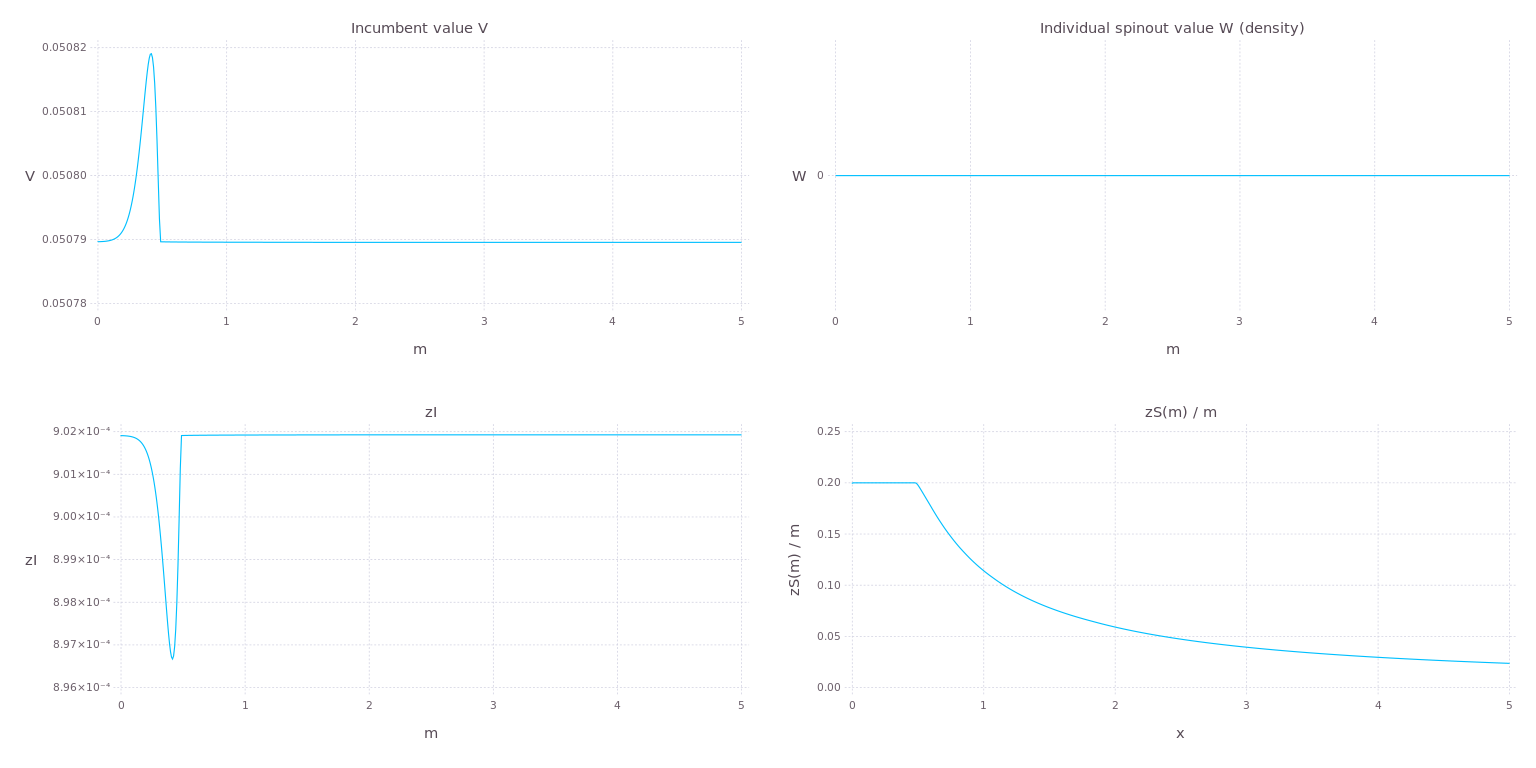
\includegraphics[scale=0.45]{../code/julia/figures/plotsGR/HJB_solutions_plot.pdf}
	\caption{Equilibrium incumbent and spinout value functions and R\&D policy.}
\end{figure}
\end{frame}

\begin{frame}{Innovation rates}
\begin{figure}
	\includegraphics[scale=0.45]{../code/julia/figures/plotsGR/innovation_rates_m.pdf}
	\caption{Equilibrium innovation rates as a function of $m$.}
\end{figure}
\end{frame}

\begin{frame}{Stationary distributions}
\begin{figure}
	\includegraphics[scale=0.45]{../code/julia/figures/plotsGR/gamma_t_mu_vs_m_plots.pdf}
	\caption{Equilibrium intermediate good distributions.}
	\label{figure:gamma_t_mu_vs_m_plots}
\end{figure}
\end{frame}

\section{Counterfactual analysis}

\begin{frame}
\tableofcontents[currentsection]
\end{frame}

\begin{frame}{Counterfactual: full enforcement of NCAs}
\begin{itemize}
\item Model calibrated assuming employers cannot use NCAs
\item Counterfactual: allow use of non-competes
\begin{itemize}
\item Welfare $\uparrow$ 1.25\%
\item Productivity growth  $\uparrow$ 3.5\% (0.05 p.p.)
\item Incumbent innovation rate $\uparrow$ 4.8\% (0.7 p.p.)
\item Non-spinout entrant innovation rate $\uparrow$ 10.5\% (0.47 p.p.)
\item Spinout innovation rate $\downarrow$ 45\% (0.45 p.p.)
\end{itemize}
\end{itemize}
\end{frame}

\begin{frame}{Equilibrium knowledge transfer}
%\centering
\begin{figure}
	\includegraphics[scale=0.45]{../code/julia/figures/plotsGR/effectiveRDWage_vs_m.pdf}
	\caption{In the calibration, unrestricted knowledge transfer to the employee harms the bilateral pair, creating a role for NCAs}
\end{figure}
\end{frame}

\begin{frame}{Equilibrium noncompete usage}
%\centering
\begin{figure}
	\centering
	\includegraphics[scale=0.45]{../code/julia/figures/plotsGR/noncompete_usage_m.pdf}
	\caption{Noncompetes are used whenever possible, given the parametrization of the model (numerical issues at edge of state space)}
\end{figure}
\end{frame}


\begin{frame}{Importance of parameters $\kappa,\theta,\nu$}
\begin{itemize}
	\item High $\kappa$ increases incumbent effective R\&D wage
	\begin{itemize}
		\item Lower value of spinout $\Rightarrow$ incumbent R\&D wage discount decreases
		\item Spinouts earn rents $\Rightarrow$ spinout entry is only slightly reduced
	\end{itemize}
	\item High $\nu , \theta$ amplify effect from $\kappa$
	\begin{itemize}
		\item High $\nu$ implies more spinouts
		\item High $\theta$ implies more WSOs
	\end{itemize}
\end{itemize}
\end{frame}

\begin{frame}{Counterfactual: reduction in entry cost $\kappa$}
\begin{itemize}
	\item Reducing entry cost $\kappa$ from $0.82$ to $0.7$ reduces welfare by 4.5\%
	\begin{itemize}
		\item Growth decreases by 3.9\% (0.06 p.p.)
		\item Incumbent innovation rate decreases 12.4\% (1.8 p.p.) 
		\item Non-spinout entrant innovation rate increases 15\% (0.75 p.p.)
		\item Spinout innovation rate decreases 46\% (.24 p.p.)
		\item Labor allocation to R\&D increases 30\% (3 p.p.)
	\end{itemize}
	\item Reduction in $\kappa$ expands PPF $\Rightarrow$ reduction in welfare implies exacerbation of market inefficiency 
	\item Underinvestment in R\&D in laissez-faire, and reducing entry cost increases R\&D spending overall, but reduces welfare (incumbents more efficient at R\&D spending)
\end{itemize}
\end{frame}


\appendix



\begin{frame}\label{spinouts_facts_from_literature}
\hyperlink{motivation_spillovers}{\beamergotobutton{back}}
\begin{itemize}
\item All spinouts
\begin{itemize}
\item More patents / R\&D, sales growth, higher survival rates (Baslandze 2019) 
\end{itemize}
\item Within-industry spinouts (WSOs)
\begin{itemize}
\item 15\% of entrants; larger at entry, grow faster, higher survival rates (Muendler et al. 2012, Brazilian data)
\end{itemize}
\end{itemize}
\end{frame}

\begin{frame}{Motivation 1: Importance of firm entry, creative destruction in productivity growth}
\begin{itemize}
	\item Accounting: firm entry contributes substantially to productivity growth
	\begin{itemize}
		\item 25\% of labor productivity growth in manufacturing (Baily-Bartelsman-Haltiwanger 1996)
		\item 25\% of aggregate productivity growth due to entrants (Akcigit-Kerr 2017)
	\end{itemize}
	\item Accounting: creative destruction constitutes the majority of firm entry
	\begin{itemize}
		\item 90-95\% of growth attributable to firm entry is due to creative destruction (Garcia-Macia, Hsieh and Klenow 2018)
	\end{itemize}
\end{itemize}
\end{frame}

\begin{frame}{Spinouts of Fairchild Semiconductor}\label{fairchildren_early}
\begin{figure}
	\includegraphics[scale=0.34]{../figures/fairchildren_early.png}
\end{figure}
\end{frame}



\begin{frame}{Incumbent HJB}\label{HJB_incumbent}
\hyperlink{closing_the_model}{\beamergotobutton{back}}
\begin{itemize}
\item Incumbent value $V(q,m,t)$ satisfies
\tiny
\begin{align*}
(\rho + \tau_E(m)& + \tau_S(m)) V(q,m,t) = \pi(q,m,t) + V_t(q,m,t) + \overbrace{\bar{\sigma}V_m(q,m,t)}^{\textrm{Spinouts from $-j$}}  \nonumber \\ 
&+ \max_{z \ge 0, x\in \{0,1\}} \Big\{ \underbrace{\chi_I z^{1-\psi} \Big[V(\lambda q,0,t) - V(q,m,t) \Big]}_{\textrm{EV of innovation}} \\
&-(1-x) z \underbrace{\Big(\frac{q}{Q(t)}\Big) \Big(  w(q,m,t) + \Big(\frac{q}{Q(t)}\Big)^{-1} \theta \nu V_m(q,m,t) \Big)}_{\textrm{Eff. cost of R\&D w/o NCA}} - xz \underbrace{\Big( \frac{q}{Q(t)} \Big) w^{NCA}(q,m,t)}_{\textrm{Cost of R\&D w/ NCA}} \Big\} 
\end{align*}
\footnotesize
where $\tau_E = \tau_E(q,m,t),\tau_S = \tau_S(q,m,t)$ and $\bar{\sigma} = \dot{m}_j^{\textrm{from } -j}$
\end{itemize}
\end{frame}


\begin{frame}{Spinout HJB}\label{HJB_spinout}
\hyperlink{closing_the_model}{\beamergotobutton{back}}
\begin{itemize}
\item Spinout value $W(q,m,t)$ satisfies
\scriptsize
\begin{align*}
(\rho  + \tau_E + \tau_S& + \tau_I)W(q,m,t) = W_t(q,m,t) + \overbrace{\big(\bar{\sigma} + \sigma(m) \big)W_m(q,m,t)}^{\textrm{Spinouts from $j$ and $-j$}}\nonumber \\
+& \max_{0 \le z \le 1} \Big\{ \underbrace{\chi_S z (z_E + z_S)^{-\hat{\psi}} (1-\kappa) V(\lambda q,0,t)}_{\textrm{Flow value of potential innovation}} - \underbrace{\Big(\frac{q}{Q(t)}\Big) z \bar{w}_t}_{\textrm{R\&D cost}} \Big\} 
\end{align*}
\footnotesize
where $\tau_K = \tau_K(q,m,t)$ for $K \in \{I,E,S\}$ and $z_E = z_E(q,m,t), z_S = z_S(q,m,t)$ and $\sigma(m) = \dot{m}_j^{\textrm{from }j}$
\end{itemize}
\end{frame}


\begin{frame}{Scaling of value functions}\label{scaling_of_value_functions}
\hyperlink{closing_the_model}{\beamergotobutton{back}}
\begin{itemize}
\item Incumbent and spinout value functions $V(q,m,t),W(q,m,t)$, entrant and spinout behavior $z_E(q,m,t),\tau_E(q,m,t),z_S(q,m,t),\tau_S(q,m,t)$ 
\item Guess and verify: BGP equilibrium with $V(q,m,t) = qV(m); W(q,m,t) = qW(m); z_E(q,m,t) = z_E(m)$ and similarly for $\tau_E,z_S,\tau_S$
\item Worker indifference condition implies $w(q,m,t) = Q(t) w(m)$ 
\end{itemize}
\end{frame}

\begin{frame}{Static equilibrium given $L_{RD}$}\label{static_eq_conditions}
\hyperlink{closing_the_model}{\beamergotobutton{back}}
\begin{itemize}
\item Final goods wage $\bar{w}(t) = \overbrace{\beta^{\beta} (1-\beta)^{1-2\beta}}^{:= C(\beta)} Q(t)$
\item Final goods production labor allocation $L_F(t) = \frac{1 - L_{RD}(t)}{1 + \big(\frac{1-\beta}{C(\beta)}\big)^{1/\beta}}$
\item Final goods production $Y(t) = \frac{(1-\beta)^{1-2\beta}}{\beta^{1-\beta}} Q(t) L_F(t)$
\item Intermediate goods firm profits $\pi(q,m,t) = (1-\beta) C(\beta) L_F(t) q $ 
\end{itemize}
\end{frame}

\begin{frame}{Aggregation}\label{aggregation}
\hyperlink{closing_the_model}{\beamergotobutton{back}}
\small
\begin{itemize}
\item Stationary density $\mu(m)$ determined by KF equation
\begin{align*}
0 = - \frac{d}{dm} \Big( \sigma(m) \mu(m) \Big) - \tau(m) \mu(m)
\end{align*}
\item Solution
\begin{align*}
\mu(m) &= C_\mu e^{-\int_0^m \frac{\sigma'(m') + \tau(m')}{\sigma(m')}dm'} 
\end{align*}
\item Conditional mean $\Gamma(m) = E[q/Q | m]$ given by 
\begin{align*}
\Gamma(m) &= \tilde{\Gamma}(s(m))
\end{align*}
where
\begin{align*}
\tilde{\Gamma}(s) &= C_{\Gamma} e^{-gs} \\
s(m) &= \int_0^m \frac{1}{\sigma(m')} dm' \\
1 &= \int_0^{\infty} \Gamma(m) \mu(m) dm
\end{align*}
\end{itemize}
\end{frame}




\begin{frame}{Aggregate distribution and BGP}\label{aggregate_distribution_and_bgp}
\hyperlink{closing_the_model}{\beamergotobutton{back}}
\begin{itemize}
\item Distribution $d\mu(q,m,t)$ shifts over time
\begin{itemize}
\item Marginal over $m$ constant over time
\item Growth in $Q(t)$ $\Rightarrow$ $\textrm{Pr}_t[q \le k | m]$ not constant
\item Proportional growth in $q$, no exit for low $q/Q(t)$ $\Rightarrow$ $\textrm{Pr}_t[q /Q(t)\le k | m]$ not constant due to "fanning out"
\item However, \textbf{\alert{conditional mean given $m$}} , $\Gamma(m;t) := E_t[q/Q(t) | m]$, constant over time
\item Sufficient for BGP given policies derived above because
\begin{itemize}
\item Individually optimal $z$ (effective R\&D) depend on $m$ only
\item R\&D labor demand given $(z,q)$ is $\frac{q}{Q}z$
\item Growth contributions aggregate $g(t) = (\lambda -1)\int_{q,m} \tau(m) \Gamma(m) \mu(m) dm$
\end{itemize}
\end{itemize}
\end{itemize}
\end{frame}


\begin{frame}{Accounting for spinouts}\label{regs_economic_significance}
\hyperlink{calibration_targets}{\beamergotobutton{back}}
\begin{figure}[!htb]
	\includegraphics[scale=0.3]{../empirics/figures/founder2_founders_f3_Accounting.pdf}
	\caption{\tiny Economic magnitude of regression estimates. The first row of figures compares the predicted number of employee founders (dotted lines) to the observed number of employee founders (solid lines). The left figure considers all founders, the right figure only founders of firms in the same 4-digit NAICS industry as their previous employers. The bottom row shows the percentage explained in each year.}
\end{figure}
\end{frame}















\end{document}